\section{Relativistic Formulation of a Free Particle}

At the end of last week, we discovered that the wave equation (in Maxwell theory) must hold in all inertial frames, and as such the notion of boosts in Maxwell theory is different from the Galilean version in classical mechanics. Today what we will do is follow Einstein, and take the attitude that all physical laws must be Lorentz invariance.

To this end, we will need to be generalize the idea of the coordinate $\v{x}(t)$. In classical mechanics, the momentum $\v{p} = m\dot{\v{x}}$ is conserved, and can take on any value. But in the relativistic theory $\abs{\dot{\v{x}}}$ is bounded above by the speed of light. Some kind of reformulation is necessary. We also have the EM fields $\v{E}(\v{x}, t), \v{B}(\v{x}, t)$ - these are already coming out of a Lorentz invariant theory, but we can rewrite the Maxwell equations such that they are manifestly Lorentz covariant.

\begin{center}
    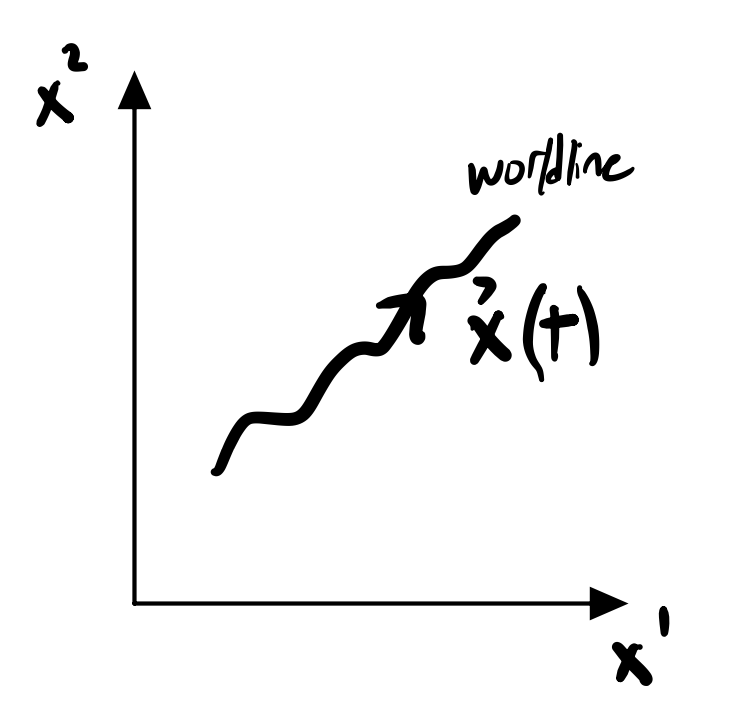
\includegraphics[scale=0.35]{Lectures/Images/lec3-worldline.png}
\end{center}

In classical mechanics, we write down the Lagrangian:
\begin{equation}
    \mathcal{L} = \frac{1}{2}m\dot{\v{x}}^2 - U(\v{x})
\end{equation}
and then solve the EL equations to find the trajectories. 

\subsection{Parametrization}
However, for a relativistically covariant formulation, we would like to put $\v{x}, t$ on the same footing. To this end, we can introduce a parameter $\lambda$, and describe the worldline of the particle as:
\begin{equation}
    x^\mu = x^\mu(\lambda)
\end{equation}
with $\mu = 0, 1, 2, 3$. This might look outlandish, but we do such parametrizations in simpler contexts. For example, consider a line in 2D space:

\begin{center}
    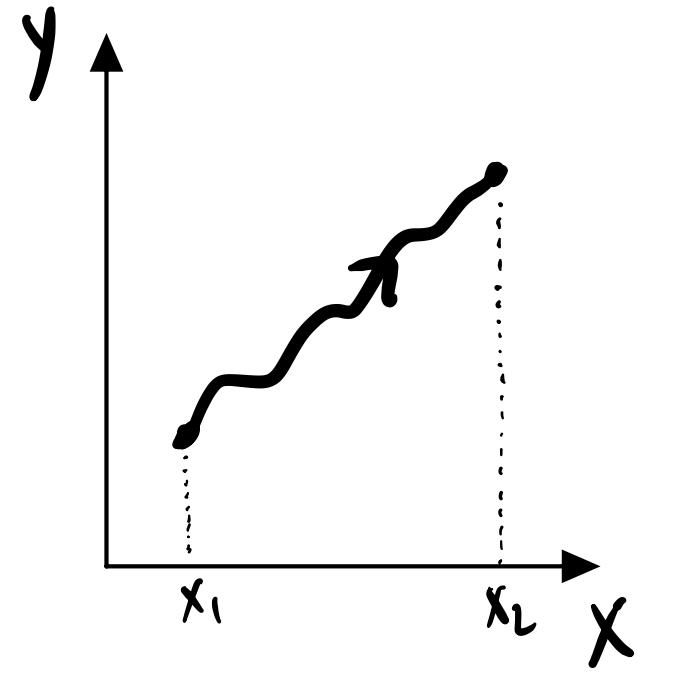
\includegraphics[scale=0.35]{Lectures/Images/lec3-yxpath.png}
\end{center}

Then we could either write $y = y(x)$, or we could write $y = y(\lambda), x = x(\lambda)$ and make them depend on a common parameter:
\begin{equation}
    x = \lambda, y = \lambda^2, \lambda \in [0, 1]
\end{equation}
In doing so, we actually introduced an additional symmetry in the form of reparametrization invariance; indeed we can have $x, y$ in terms of an arbitrary (monotonic, positive) function of $\lambda$:
\begin{equation}
    x= f(\lambda), y = f^2(\lambda), \lambda \in [0, 1]
\end{equation}
This can be useful for calculations in various contexts. For example, suppose we were interested in calculating the length of the line:

\begin{center}
    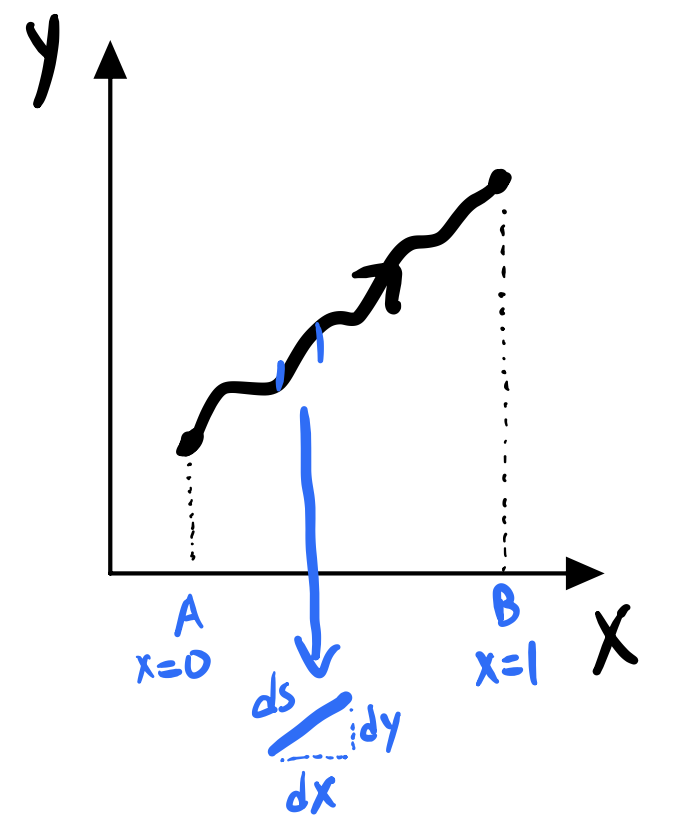
\includegraphics[scale=0.35]{Lectures/Images/lec3-lineelement.png}
\end{center}

Then:
\begin{equation}
    L = \int_A^B ds = \int_A^B \sqrt{dx^2 + dy^2} = \int_0^1 dx \sqrt{1 - \left(\dod[]{y}{x}\right)^2} = \int_0^1 dx\sqrt{1 + y'^2}
\end{equation}

But if $x = x(\lambda), y = y(\lambda)$ for some parameter $\lambda$, we could then write:
\begin{equation}
    ds^2 = (dx(\lambda))^2 + (dy(\lambda))^2 = \left(\dod{x}{\lambda}d\lambda\right)^2  + \left(\dod{y}{\lambda}d\lambda\right)^2 = d\lambda^2\left(\dot{x}^2 + \dot{y}^2\right)
\end{equation}
So:
\begin{equation}
    L = \int_A^B ds = \int_A^B \sqrt{d\lambda^2\left(\dot{x}^2 + \dot{y}^2\right)} = \int_A^B d\lambda\sqrt{\dot{x}^2 + \dot{y}^2}
\end{equation}
the length calculation is now symmetric in $x, y$. If we replace $\lambda \to f(\lambda)$, the length should not change (for it shouldn't matter on the parameterization of the curve!) This must be a symmetry of the integral, and indeed we can easily check that it is. Under $\lambda \to f(\lambda)$:
\begin{equation}
    x^\mu = \frac{dx^\mu}{d\lambda} \to \frac{dx^\mu}{df(\lambda)} = \frac{dx^\mu}{d\lambda}\frac{d\lambda}{df(\lambda)}
\end{equation}
and the same for $y^\mu$. Thus the length becomes:
\begin{equation}
    L = \int_A^B df(\lambda)\sqrt{\left(\frac{dx^\mu}{df(\lambda)}\right)^2 + \left(\frac{dy^\mu}{df(\lambda)}\right)^2} = \int_A^B d\lambda \dot{f} \sqrt{\left(\frac{\dot{x}}{\dot{f}}\right)^2 + \left(\frac{\dot{y}}{\dot{f}}\right)^2} = \int_A^B d\lambda\sqrt{\dot{x}^2 + \dot{y}^2}
\end{equation}
which we can see is invariant (as it should be).

\subsection{Parametrizing Worldlines and Time Dilation}
Back to our problem of parametrizing worldlines. We can repeat the idea from the simple context here, by describing the particle worldine as $x^\mu(\lambda)$. Other than the fact that the time component has a different sign:
\begin{equation}
    ds^2 = -(dx^0)^2 + (dx^1)^2 + (dx^2)^2 + (dx^3)^2
\end{equation}
we can play the same game as before; with $x^\mu = x^\mu(\lambda)$:
\begin{equation}
    ds^2 = d\lambda^2\left(-(\dot{x}^0)^2 + (\dot{x}^1)^2 + (\dot{x}^2)^2 + (\dot{x}^3)^2\right) = d\lambda^2 \dot{x}^\mu \dot{x}_\mu = d\lambda^2 \dot{x}^\mu \dot{x}^\nu \eta_{\mu\nu}
\end{equation}
This line element is reparametrization invariant, but also is Lorentz invariant (as it is written as a contraction with the Minkowski metric).

To do physics, we want to fix reparametrization symmetry. It is natural to fix $x^0(\lambda) = \lambda c$, so then $t(\lambda) = \lambda$. The logic is we have four functions, and we can freely reparametrize - using this symmetry, we may pick the time function to be simple. Let's see what happens to $ds^2$ when we do this:
\begin{equation}
    ds^2 = dt^2\left(-c^2 + \left(\dod{\v{x}}{t}\right)^2\right) = -c^2dt^2\left(1 - \gv{\beta}^2\right)
\end{equation}
with $\gv{\beta} = \frac{\v{v}}{c} = \frac{\dot{\v{x}}}{c}$. A natural definition is:
\begin{equation}
    d\tau^2 = dt^2(1 - \gv{\beta}^2)
\end{equation}
so:
\begin{equation}
    ds^2 = -c^2d\tau^2
\end{equation}
$\tau$ is called the proper time. In the frame where $\gv{\beta} = 0$, we can see from the above $\tau = t$; it thus has the interpretation as the time in the inertial frame in which the particle is at rest momentarily. The relation between $t, \tau$ can be written as:
\begin{equation}
    dt = \gamma d\tau
\end{equation}
with:
\begin{equation}
    \gamma^2 = \frac{1}{1 - \gv{\beta}^2}
\end{equation}
This is the celebrated time dilation formula. This says that things that take time $d\tau$ in the frame of the particle are dilated/increased by $\frac{1}{1-\gv{\beta}^2}$ in the frame of the external observer. As a concrete example, if a particle has a lifetime $T$, someone who sees the particle moving will see its lifetime as $\gamma T$. You may be familiar with the fact that cosmic rays create muons with, $T = 2.2 \cdot 10^{-6}\si{s}$. In the muon frame, it can only travel $2. 2 \cdot 10^{-6}\si{s} \cdot 3 \times 10^{8}\si{ms^{-1}} = 0.66\si{km}$. But we observe that cosmic ray muons propagate for hundreds of kilometers, and the explanation is that their lifetime is extended via time dilation.

\subsection{Lagrangian for Relativistic Particle}
The usual Lagrangian:
\begin{equation}
    \mathcal{L} = \frac{1}{2}m\dot{\v{x}}^2 - U(\v{x})
\end{equation}
does not work in our relativistic formulation as the particle could have any velocity, and velocities are bounded by the speed of light. Further, the action $S = \int dt \mathcal{L}$ is not invariant under Lorentz transformations. Can we modify this Lagrangian in some way? A very natural candidate is:
\begin{equation}\label{eq:LIaction}
    S = A\int d\lambda \sqrt{-\dot{x}_\mu \dot{x}^\mu}.
\end{equation}
This is automatically Lorentz invariant. It is also reparametrization invariant, so let us fix the reparametrization symmetry by taking $\lambda = t$:
\begin{equation}
    S = \tilde{A}\int dt \sqrt{1 - \frac{\dot{\v{x}^2}}{c^2}}.
\end{equation}
This is now invariant under the boosts that we defined last week - even though it looks like it mixes $x/t$ because they are written separately, we know from the form of Eq. \eqref{eq:LIaction} that it is indeed invariant. It is also now clear why we took the minus sign there; we want the argument of the square root to be always positive.

We are not quite done yet. We have to check that the action passes basic scrutiny. One sanity check is that in the non-relativistic limit of $\dot{\v{x}} \ll c$. Using the binomial approximation:
\begin{equation}
    S = \tilde{A}\int dt\left[1 - \frac{1}{2}\frac{\dot{\v{x}}^2}{c^2} + O(\frac{\abs{\dot{\v{x}}}^4}{c^4})\right]
\end{equation}
This motivates the choice that $\tilde{A} = -mc^2$:
\begin{equation}
    S = \int dt\left(-mc^2 + \frac{1}{2}m\dot{\v{x}}^2 + \ldots \right)
\end{equation}
This looks very good! We have the kinetic term with the correct normalization, and the first term can be thought of the rest energy of the particle $U = mc^2$. Note that the zero of the energy has been fixed - in regular classical mechanics, we usually have a freedom to choose what our ``zero'' is, but it does matter here.

The bottom line is our action:
\begin{equation}
    S = -mc^2\int dt\sqrt{1 - \frac{\dot{\v{x}}^2}{c^2}}
\end{equation}
has the properties that it is Lorentz invariant and it produces the correct formula in the low-velocity limit. This is the action we will be working with!

\subsection{Relavistic energy and momentum}

We want to turn the crank of the classical mechanics machinery and write down the Euler-Lagrange equations, and define energy and momentum. The E-L equations are:
\begin{equation}
    \dod{}{t}\ddpd{\LL}{\dot{x}^i} = \ddpd{\LL}{x^i}
\end{equation}
for $i = 0$. Since the Lagrangian is independent of $x^i$:
\begin{equation}
    \dod{}{t}\ddpd{\LL}{\dot{x}^i} = 0
\end{equation}
Thus we can define the (conserved) momentum:
\begin{equation}
    p^i = \frac{m\dot{x}^i}{\sqrt{1-\frac{\v{v}^2}{c^2}}} = \gamma m\dot{x}^i
\end{equation}
So the difference between the non-relativistic case ($m\dot{x}^i$) and relativistic case ($\gamma m\dot{x}^i$) is that $\gamma m$ is an effective ``relativistic mass''; the faster the particle travels, the heavier it becomes/harder it becomes to change its momentum (and hence it can never surpass the speed of light).

We can also write down the Hamiltonian (equal to the energy because $\LL$ does not depend on time):
\begin{equation}
    H = E = p_i \dot{x}^i - \LL = \gamma mc^2
\end{equation}
where again the energy becomes larger and larger the more the particle approaches the speed of light.

You can easily convince yourself that:
\begin{equation}\label{eq:Eprelation}
    E^2 = c^2\abs{\v{p}}^2 + (mc^2)^2
\end{equation}
This is an interesting formula for the following reason. $(E, \v{p})$ are a scalar and vector under rotations. Because rotations are a subgroup of Lorentz transformations, they presumably can be combined to a four-vector $p^\mu = (\frac{E}{c}, \v{p})$. $p^\mu \to p'^\mu = \Lambda^{\mu}_{\sp\nu}p^\nu$ under Lorentz transformations. In this language, Eq. \eqref{eq:Eprelation} has the nice inrepretation:
\begin{equation}
    p_\mu p^\mu = -(mc)^2
\end{equation}
So the combination $p_\mu p^\mu$ is a Lorentz invariant quantity.

Next time, we will look at the relativistic formulation of Maxwell's theory; we have fields $\v{E}(\v{x}, t), \v{B}(\v{x}, t)$, which satisfy:
\begin{equation}
    \nabla \cdot \v{E} = \frac{\rho}{\e_0}
\end{equation}
\begin{equation}
    \nabla \cdot \v{B} = 0
\end{equation}
\begin{equation}
    \nabla \times \v{B} - \frac{1}{c}\v{E} = \mu_0 \v{J}
\end{equation}
\begin{equation}
    \nabla \times \v{E} + \dot{\v{B}} = 0
\end{equation}
we will repackage these in such a way that it is clearer to see that they are Lorentz invariant. We will then combine our work on a relativistically invariant formulation of the mechanics of a particle with this.